\chapter{Results}
\section{Available evidence and execution status}
The real descriptor table passes the implemented schema, finite-value, replica and interval checks. Each of the three segments contains \num{100001} rows at the source-labelled 20 ps spacing. Thus the data are suitable for the reported scalar-descriptor diagnostics, subject to the provenance assumptions described earlier. This validation does not independently establish simulation convergence or the correctness of upstream molecular definitions.

The reported diagnostics come from run \code{\DiagnosticRun}. Its recorded elapsed time is \DiagnosticSeconds{} s, and its sampled peak worker-process memory is \DiagnosticMemory{} MiB. These measurements describe this lightweight local run only. They are not estimates of full DPC runtime, nor evidence of HPC execution. The earlier reproduction attempt stopped at the missing-FES gate. Subsequent complete-grid validation and the independent GMM run have distinct manifests and do not convert that blocked attempt into a successful reproduction.

\begin{table}[htbp]
\centering
\begin{tabularx}{\textwidth}{@{}lX@{}}\toprule
Analysis & Evidence status\\\midrule
Input validation & Completed on the supplied Aβ40 descriptor table\\
Correlation matrix / PCA & Completed; unweighted biased-sample diagnostics\\
Autocorrelations / provisional ESS & Completed; every estimate flagged as unreliable\\
FES grid and interpolation & Completed; units/construction remain unverified\\
Weighted paper reproduction & Blocked: unit/construction provenance\\
GMM seed / SASA-ablation pilot & Completed; biased-sample geometric comparison\\
DPC seed / feature / scaling studies & Not completed; separate reproduction prerequisites\\
Time-dependent weight comparison & Blocked: FES and rbias unit/provenance requirements\\
Molecular representatives / ShapeGMM & Blocked: coordinate trajectory and mapping absent\\
External validation / Leonardo jobs & Not performed\\\bottomrule
\end{tabularx}
\caption{Scientific evidence available at release. Tests on synthetic fixtures are excluded from the empirical analysis statuses.}
\label{tab:status}
\end{table}

\section{Descriptor distributions and redundancy}
The pooled Rg--SASA Pearson correlation is \RgSasaCorrelation{}, whereas the correlation between the two secondary-structure descriptors is \AlphaBetaCorrelation{}. These are properties of the biased observation sample. The strong compaction/exposure correlation motivates a SASA-ablation experiment, but does not demonstrate that either variable is dispensable for every local family.

The first standardized principal component explains \PCAFirst{}\% of total variance, and the second explains \PCASecond{}\%, giving \PCATwo{}\% cumulatively. \Cref{fig:features} presents the numerical correlation matrix and spectrum. This concentration of variance supports examining redundant directions; it does not justify discarding a lower-variance variable without checking the effect on clustering and relevance.

\begin{figure}[htbp]
\centering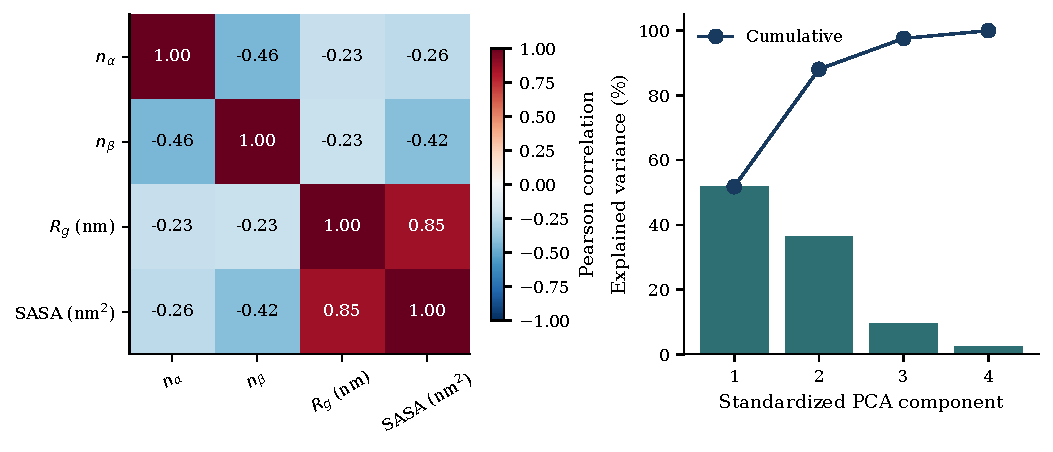
\includegraphics[width=\textwidth]{fig03_feature_diagnostics.pdf}
\caption{Computed diagnostics for the pooled, unweighted Aβ40 descriptor sample. Left: Pearson correlations of the four baseline descriptors. Right: explained variance of PCA after per-feature standardization, with cumulative variance shown by the line. These are geometric summaries of the biased sample and do not represent reweighted equilibrium probabilities.}
\label{fig:features}
\end{figure}

\Cref{fig:rawdistributions} shows per-replica empirical densities on common descriptor-specific bin edges. Each histogram is normalized by its own frame count and bin width. Differences between replicas are visible, but their equilibrium significance cannot be determined from these raw distributions alone. The plotted densities therefore describe the sampled trajectories, with no equilibrium correction.

\begin{figure}[htbp]
\centering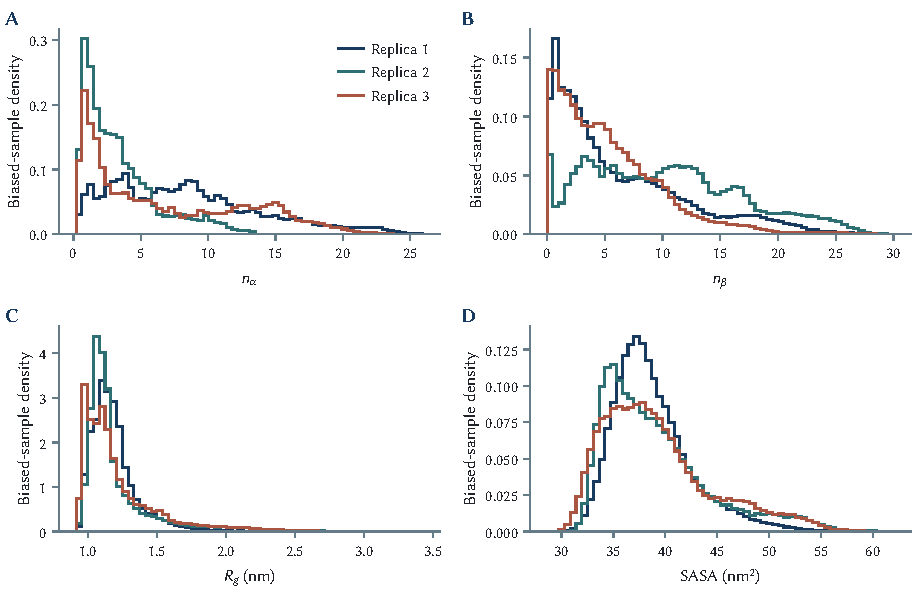
\includegraphics[width=.95\textwidth]{raw_descriptor_distributions.pdf}
\caption{Actual per-replica descriptor histograms over the supplied interval. Curves use common bin edges for each descriptor and independent density normalization. No final-bias or time-dependent statistical weights have been applied. Units follow the original script's labels and remain a recorded upstream-provenance assumption.}
\label{fig:rawdistributions}
\end{figure}

\section{Temporal correlation and provisional ESS}
The correlation diagnostics produce provisional ESS values ranging from \ESSMinimum{} to \ESSMaximum{} across the 12 replica--descriptor series, compared with \num{100001} raw frames in each series. All \UnreliableCount{} estimates fail at least one configured reliability heuristic. They should therefore be read as warning indicators of strong dependence and possible nonstationarity, not as precise counts of independent equilibrium conformations.

\Cref{tab:sampling} reports the estimator outputs together with the half-window mean shift. Several descriptors exhibit substantial differences between the first and second halves of the recorded interval. The extension does not convert those shifts into a formal rejection of the published convergence analysis, because the full bias history and corresponding convergence diagnostics are unavailable. It establishes that naive independent-frame uncertainty estimates would be poorly supported by the supplied stream.

\begin{table}[htbp]
\centering\small
\begin{tabular}{@{}clrrrr@{}}\toprule
Replica & Descriptor & $g$ & $\tau_{\mathrm{int}}$ (ns) & $N_{\mathrm{eff,corr}}$ & Half shift / SD\\\midrule
1 & $n_\alpha$ & 22067 & 220.7 & 4.5 & 1.28 \\
1 & $n_\beta$ & 11079 & 110.8 & 9.0 & 0.83 \\
1 & $R_g$ & 3679 & 36.8 & 27.2 & 0.27 \\
1 & SASA & 3490 & 34.9 & 28.7 & 0.36 \\
2 & $n_\alpha$ & 6259 & 62.6 & 16.0 & 0.37 \\
2 & $n_\beta$ & 10843 & 108.4 & 9.2 & 0.41 \\
2 & $R_g$ & 3951 & 39.5 & 25.3 & 0.33 \\
2 & SASA & 5325 & 53.2 & 18.8 & 0.17 \\
3 & $n_\alpha$ & 31742 & 317.4 & 3.2 & 1.61 \\
3 & $n_\beta$ & 5880 & 58.8 & 17.0 & 0.71 \\
3 & $R_g$ & 6259 & 62.6 & 16.0 & 0.88 \\
3 & SASA & 9958 & 99.6 & 10.0 & 0.87 \\
\bottomrule\end{tabular}

\caption{Computed correlation diagnostics. All entries are flagged as unreliable under the stated heuristics. The time scale is measured along the biased trajectory, using the source-labelled sampling interval. $g$ is statistical inefficiency; the final column is the absolute difference of half-window means divided by the full-series standard deviation. No physical relaxation-time interpretation is made.}
\label{tab:sampling}
\end{table}

\begin{figure}[htbp]
\centering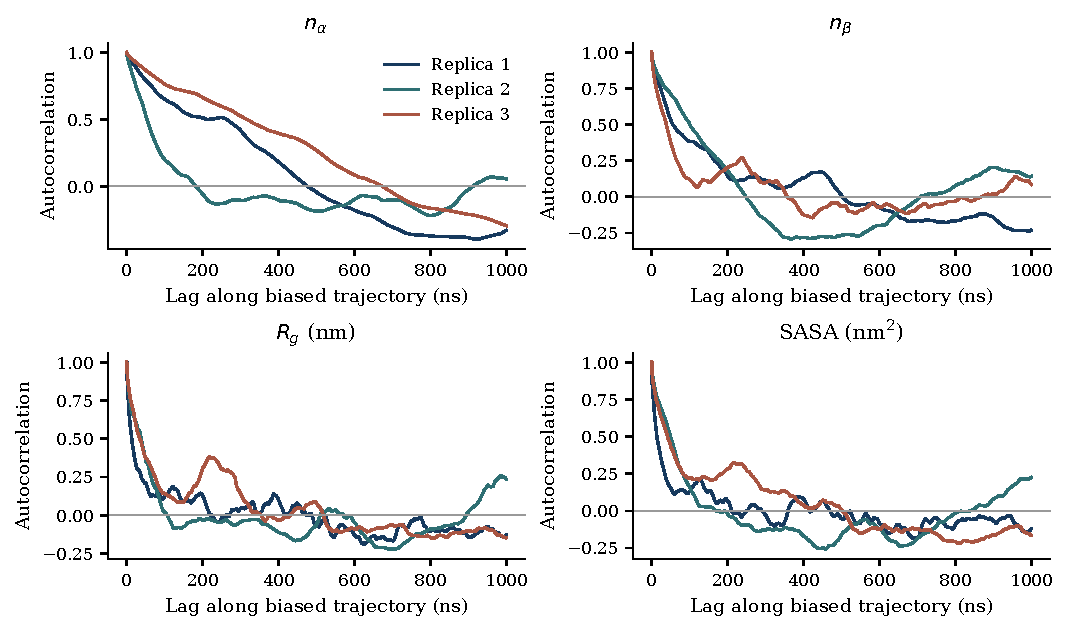
\includegraphics[width=.95\textwidth]{sampling_autocorrelations.pdf}
\caption{Autocorrelation functions computed separately for each replica and descriptor. The plotted curves cover the first half of the available lag window with a reduced plotting density; the estimator operates on the full, un-decimated ACF sequence. Long persistence and changing behavior across replicas reinforce the need for cautious uncertainty analysis. Lag is biased trajectory time, not recovered physical time.}
\label{fig:acf}
\end{figure}

\section{Complete FES validation}
The recovered file contains exactly 2,801 by 1,301 grid points: 3,644,101 rows with five finite columns, no duplicate coordinates and complete Cartesian coverage. Its nonperiodic axes span 0--28 and 0--13 at spacing 0.01. All 300,003 converted descriptor queries lie within those bounds, and bounded bilinear interpolation returns finite values for every query. The grid check is an input-integrity result; the energy column has no declared unit and is not assigned one solely because the source script assumes kJ/mol.

\section{Representation and initialization sensitivity}
The GMM pilot fitted \GMMModels{} models, all reporting convergence, in \GMMSeconds{} s with a sampled process-tree peak of \GMMMemory{} MiB. Convergence here means that the configured numerical stopping criterion was met, not that every model found the same or globally optimal solution. The comparison in \cref{fig:gmm} reveals substantial differences between component counts.
\begin{figure}[htbp]
\centering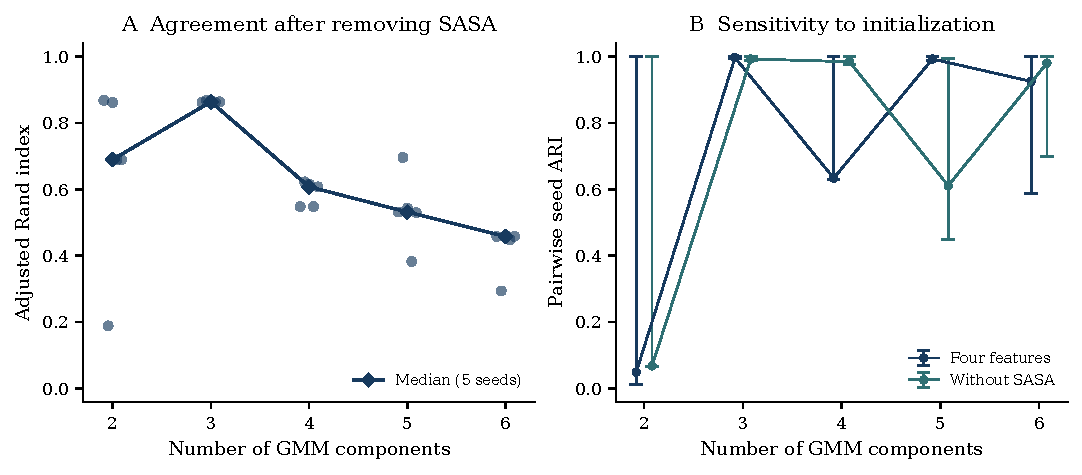
\includegraphics[width=\textwidth]{gmm_sensitivity.pdf}
\caption{Independent GMM sensitivity experiment on the biased descriptor sample. Left: four-feature versus SASA-ablated assignments at each of five seeds; diamonds mark medians. Right: within-space ARI over ten seed pairs; bars span observed minima and maxima, not confidence intervals. The fit subset is fixed across all models and evaluation includes fit rows.}
\label{fig:gmm}
\end{figure}
\begin{table}[htbp]\centering
\begin{tabular}{@{}crr@{}}\toprule Components & Median ablation ARI & Observed range\\\midrule
2 & 0.690 & 0.188--0.868 \\
3 & 0.864 & 0.862--0.868 \\
4 & 0.607 & 0.548--0.622 \\
5 & 0.531 & 0.382--0.696 \\
6 & 0.457 & 0.294--0.461 \\
\bottomrule\end{tabular}

\caption{Observed representation agreement across five paired initializations. Component count was varied by design; the table does not identify an optimal biological family count.}
\label{tab:gmm}
\end{table}
At three components, cross-representation ARI lies between 0.862 and 0.868, with approximately 95.3\% of frames retaining corresponding labels after maximum-overlap matching (median across seeds). Within-space seed agreement is also high: 0.994--1.000 with four descriptors and 0.988--1.000 without SASA. At two components, however, within-space ARI ranges down to 0.011 and 0.067, respectively. A single initialization would conceal this variability. The full matrices are retained in \cref{fig:seedmatrices}.

SASA removal preserves much of the three-component partition in this pilot, while agreement is lower or more variable at the other component counts. Thus the effect of removing SASA depends on the resolution and initialization of the fitted model. These comparisons concern assignments in the biased sample; weighted relevance and equilibrium populations have not been estimated.

\section{Analyses remaining unavailable}
Equilibrium cluster relevance, weighted family characterization and completed paper-DPC robustness remain unavailable. No molecular snapshots are created because the descriptor table has no atomic coordinates. The completed GMM experiment is an original descriptor-space extension, not a replacement for those stages.
